\chapter{Questo è un capitolo}

\lipsum[1]

\section{Questa è una sezione}

\lipsum[2]

\subsection{Questa è una sottosezione}

\lipsum[3]

\subsubsection{Questa è una sotto-sottosezione}

\lipsum[4]

É possibile riferire l'immagine, una volta assegnatagli una label, tramite il comando \texttt{\textbackslash autoref\{fig:immagine\}}, ottenendo il seguente risultato: \autoref{fig:immagine}.

\begin{figure}
    \centering
    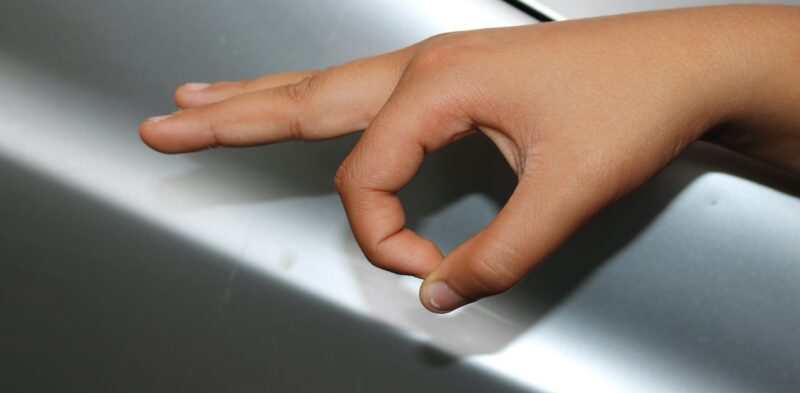
\includegraphics[width= 0.8\textwidth]{images/Capitolo1/immagine.jpg} 
    \caption{Questa è un'immagine} 
    \label{fig:immagine}
\end{figure}

Questa è una citazione \cite{LabelPerLaCitazione}.

\subsubsection{Questa è un'altra sottosezionelipsum}

Quello che segue è un esempio di codice. E' possibile modificare il linguaggio per il synyax highlight, aggiungere parole chiave... E' tutto disponibile nella guida del pacchetto \texttt{listings}.

\lstinputlisting[language=C++]{listings/Capitolo1/code1.cpp} 

\section{Questa è un'ennesima sezione}

\lipsum[4]

\subsection{Sottosezione con una tabella}

La tabella si indirizza sempre con l'uso di una label, ottenendo il risultato \autoref{tab:labelTabella}.

\begin{table}
    \caption{Una simpatica tabella!}\label{tab:labelTabella}
    \begin{center}
    \begin{tabular}{c|c|c|c}
        \textbf{Colonna 1} & \textbf{Colonna 2} & \textbf{Colonna 3} & \textbf{Colonna 4} \\
        \hline
            $3$      & $24$     & $24$    & $29$ \\ 
            $36$     & $31$     & $49$    & $39$ \\ 
            $32$     & $41$     & $59$    & $57$ \\ 
            $34$     & $60$     & $79$    & $74$ \\ 
            $328$    & $96$     & $194$   & $99$ \\ 
            $356$    & $117$    & $297$   & $149$ \\ 
            $312$    & $315$    & $293$   & $242$ \\ 
            $3024$   & $184$    & $253$   & $019$ \\ 
            $3048$   & $7795$   & $253$   & $077$ \\ 
            $3096$   & $7767$   & $2432$  & $0514$ \\ 
            $3192$   & $3769$   & $2435$  & $0551$ \\ 
            $36384$  & $6625$   & $3432$  & $0497$ \\ 
            $32768$  & $15469$  & $6472$  & $0471$ \\ 
            $35536$  & $15425$  & $14539$ & $10289$ \\ 
            $331072$ & $34623$  & $24941$ & $20444$ \\  
        \end{tabular}
    \end{center}
\end{table}